% Fig 3 (PediatricADRHAN model) - source for the submitted Fig3.tif.
% PLOS ONE figure rules: Arial, Times or Symbol font in 8-12 point, and no vector
% EPS generated in LaTeX. This version uses Liberation Sans (metrically identical
% to Arial), all text is 8-10 pt at the printed size (scale 1, no resizing), and
% the PDF is converted to TIFF:
%   xelatex Fig3_PediatricADRHAN.tex
%   pdftoppm -r 600 -png Fig3_PediatricADRHAN.pdf fig3   (then save as RGB TIFF, LZW)
\documentclass[tikz,border=2mm]{standalone}
\usepackage{fontspec}
\setmainfont{Liberation Sans}
\setsansfont{Liberation Sans}
\usepackage{xcolor}
\usetikzlibrary{positioning,arrows.meta,shadows.blur,fit}

\definecolor{jbrand}{RGB}{15,58,102}
\definecolor{jbrandlight}{RGB}{232,240,247}
\definecolor{jgrey}{RGB}{90,90,90}
\definecolor{jamber}{RGB}{176,98,10}
\definecolor{jamberlight}{RGB}{250,240,224}

\newcommand{\boxtext}{\fontsize{9}{11}\selectfont}
\newcommand{\boxtitle}{\fontsize{10}{12}\selectfont\bfseries}
\newcommand{\sidetext}{\fontsize{8.5}{10}\selectfont\itshape}

\begin{document}
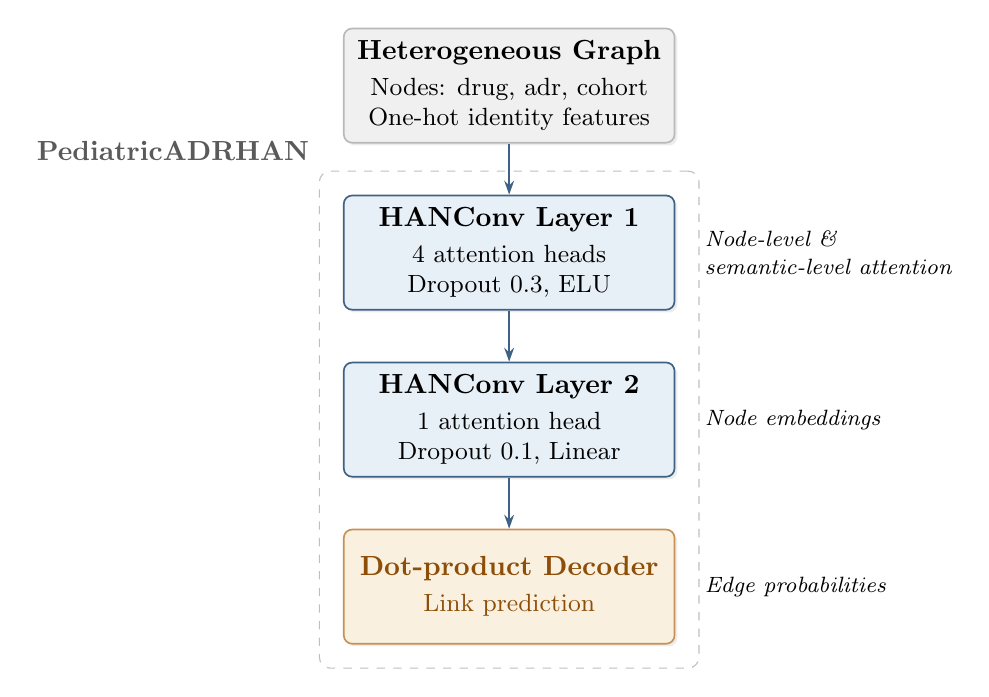
\begin{tikzpicture}[
  font=\boxtext,
  pipebox/.style={rectangle,rounded corners=3pt,draw=jbrand!80,fill=jbrandlight,
    minimum width=4.2cm,minimum height=1.45cm,align=center,line width=0.6pt,
    drop shadow={shadow xshift=1pt,shadow yshift=-1pt,opacity=0.15}},
  layerbox/.style={pipebox,fill=gray!12,draw=gray!55},
  gatebox/.style={pipebox,fill=jamberlight,draw=jamber!70,text=jamber!80!black},
  arr/.style={-{Stealth[length=5pt,width=3.5pt]},line width=0.9pt,color=jbrand!80},
]

\node[layerbox] (INPUT) at (0,0) {{\boxtitle Heterogeneous Graph}\\[2pt]Nodes: drug, adr, cohort\\One-hot identity features};
\node[pipebox, below=0.65cm of INPUT] (L1) {{\boxtitle HANConv Layer 1}\\[2pt]4 attention heads\\Dropout 0.3, ELU};
\node[pipebox, below=0.65cm of L1] (L2) {{\boxtitle HANConv Layer 2}\\[2pt]1 attention head\\Dropout 0.1, Linear};
\node[gatebox, below=0.65cm of L2] (DEC) {{\boxtitle Dot-product Decoder}\\[2pt]Link prediction};

\draw[arr] (INPUT) -- (L1);
\draw[arr] (L1) -- (L2);
\draw[arr] (L2) -- (DEC);

\node[font=\sidetext, right=0.25cm of L1, align=left] {Node-level \&\\semantic-level attention};
\node[font=\sidetext, right=0.25cm of L2, align=left] {Node embeddings};
\node[font=\sidetext, right=0.25cm of DEC, align=left] {Edge probabilities};

\node[rectangle, draw=gray!50, dashed, rounded corners, fit=(L1) (L2) (DEC), inner sep=0.3cm] (MODEL) {};
\node[above left, font=\boxtitle, text=jgrey] at (MODEL.north west) {PediatricADRHAN};

\end{tikzpicture}
\end{document}
